\section{Qualitative recalibration and the role of SSIM}
\label{sec:quality_recalibration}
\paragraph{The intended preservation target.}
The revised target retains the same main objects and scene while allowing minor appearance changes. It does not require pixel identity, but excludes missing main objects, added important people, replacement of objects and major scene changes. We inspect all 32 validation pairs from the original model's unregularized 500-update attack, omitting metric values and owner decisions from the displayed panels. Six comparisons receive native-resolution closeups. Under the clarified target, assistant visual inspection assigns 19 acceptable, 11 unacceptable and two ambiguous judgements. These are model-assisted judgements rather than independent human annotations.

\paragraph{The first numerical revision.}
A small grid varies LPIPS limits in $\{0.2,0.25,0.3,0.35\}$, SSIM minima in $\{0.5,0.6\}$, image-image CLIP minima in $\{0.85,0.9,0.95\}$ and class-retention minima in $\{0.8,0.85,0.9,0.95\}$. Balanced classification error on the 30 unambiguous judgements selects a class-retention minimum of $0.90$, rather than $0.95$, leaving the other three bounds unchanged. Ties favor fewer unacceptable edits admitted and then the smallest change from the old rule. On these fitting images, the revised rule accepts 13/19 judged acceptable edits, versus 11/19 previously, while excluding all 11 judged unacceptable. It still rejects six acceptable edits. This small in-sample calibration does not validate a general perceptual criterion. The initial interpretation, clarified user preference, ambiguous cases and grid results remain in the calibration receipts.

\paragraph{Why an absolute worst case cannot justify removing every check.}
Among watermark-evading outputs of the latest original-model attack, the worst LPIPS case loses much of a clock's casing and gains large artifacts. Another case is worst in SSIM, image CLIP and class retention; it loses an ornate foreground structure and changes the scene. These are meaningful content failures. At the other extreme, a fruit-market scene fails only SSIM, with $0.59697<0.6$, despite retaining its main objects and framing. A threshold boundary is not itself evidence of unacceptable content change.

\paragraph{Inspecting the incremental SSIM exclusions.}
To examine SSIM specifically, we retain the other three checks and inspect \emph{all nine} outputs excluded only by SSIM across both full-training studies and all three supplied models. Selection does not depend on watermark detection. The lowest SSIM is $0.56495$; its broken-tile scene retains the same main objects despite changes to local geometry and texture. The other eight pairs also retain their main scene under the stated tolerance, including ceiling artwork, timber and fruit displays. This informal visual review motivates removing SSIM from the mandatory conjunction, while continuing to report it. It does not establish that SSIM is redundant for other data or that every local detail is preserved. Because these are already evaluated final outputs, this additional decision and all resulting comparisons are explicitly post-hoc.

The current diagnostic requires finite metrics, LPIPS at most $0.2$, image-image CLIP at least $0.9$ and class-alignment retention at least $0.9$. The owner threshold remains strict bit accuracy $>0.6875$. Source and raw PNG hashes are checked against the final artifact freezes. Before changing any quality decision, the analysis exactly reconstructs every old raw and returned outcome for all six model/study combinations. No generator is retrained, no owner threshold is fitted and no old result is overwritten.

\begin{table}[ht]\centering\small
\begin{tabular}{llrrr}\toprule
\shortstack{Inner\\steps} & Model & \shortstack{Historical\\joint} & \shortstack{Retained\\joint} & \shortstack{Candidate\\pass}\\\midrule
100 & original & 20/64 & 28/64 & 33/64\\
100 & fixed & 22/64 & 26/64 & 31/64\\
100 & adapted & 22/64 & 31/64 & 35/64\\
500 & original & 20/64 & 29/64 & 30/64\\
500 & fixed & 21/64 & 28/64 & 30/64\\
500 & adapted & 20/64 & 28/64 & 30/64\\
\bottomrule\end{tabular}
\caption{Post-hoc preservation reanalysis of open-weight DistSeal UViT-H/DC-AE clean-training attacks, with 64 paired inputs per row. Inner steps gives the clean adaptation horizon used in training the defense candidates. Original is the released marked generator; Fixed and Adapted are the meta-distilled reference variants. Historical joint uses LPIPS $\leq0.2$, SSIM $\geq0.6$, image CLIP $\geq0.9$ and class retention $\geq0.95$. Retained joint uses LPIPS $\leq0.2$, image CLIP $\geq0.9$ and class retention $\geq0.9$. Candidate pass counts raw adapted images passing the retained rule before any source fallback. Joint counts simultaneous preservation and loss of owner detection at bit accuracy $\leq0.6875$. The two horizons have different generation seeds; comparisons are paired within each horizon. This reuses evaluated data.}\end{table}


For the 500-inner-step revision, quality-preserving removals are now 29/64 for the released model and 28/64 for each trained variant. Raw preservation passes are 30/64 for all three. The original frozen rule gave 20/64, 21/64 and 20/64 joint removals; the intermediate class-only revision gave 27/64, 25/64 and 25/64. The client can still return its marked source when the raw edit fails the remaining gates, so its raw generator does not preserve every source image. Both variants improve the removal-rate point estimate by only $1.5625$ percentage points relative to the original. Descriptive paired 95\% bootstrap intervals are $[-7.81,4.69]$ points for fixed reference and $[-6.25,3.13]$ for adapted reference. Both include zero: this is not a confirmed defense gain.

The 100-inner-step study gives 28/64, 26/64 and 31/64 joint removals under the same current rule. Its generation seeds differ from the 500-step study, so each variant must be compared to its own original-model baseline. A separate quality-selected LoRA attack removed 0/64 watermarks from each model, including the original. The original, fixed and adapted arms preserved 64/64, 60/64 and 59/64 images, respectively. With no baseline removals, this pilot cannot distinguish defense strength. Its compact receipt remains in \path{tex/provenance/discarded_lora_run.json}. All revised comparisons reuse previously evaluated images and are not fresh confirmation or independent human-quality validation.

\begin{figure}[p]\centering
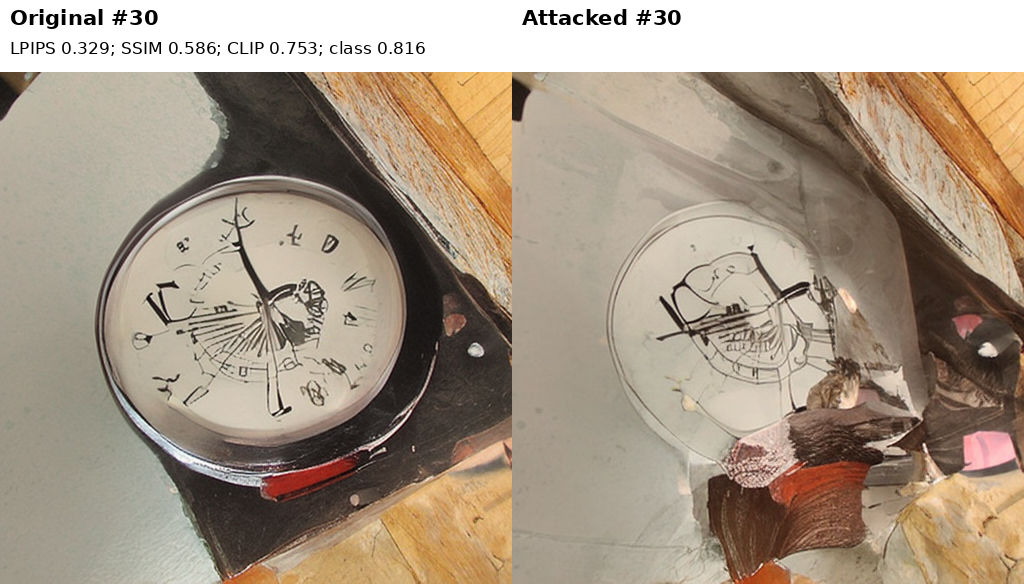
\includegraphics[width=.98\linewidth]{figures/worst-quality-evasion-30.png}
\caption{The worst LPIPS watermark-evading example from the latest original-model attack. The clock casing and surrounding structure change substantially. Removing all preservation checks would admit a visibly changed source.}
\end{figure}
\begin{figure}[p]\centering
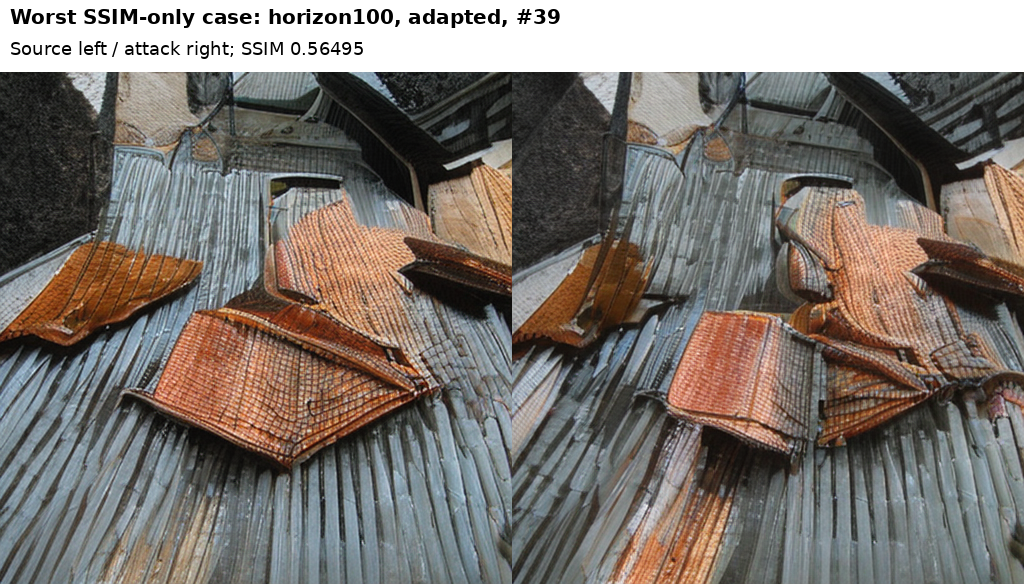
\includegraphics[width=.98\linewidth]{figures/ssim-only-worst.png}
\caption{The lowest SSIM among every SSIM-only rejection in both studies, irrespective of watermark outcome. Under the stated main-object and scene criterion, local texture and geometry changes are permitted. The remaining three gates pass.}
\end{figure}

The other eight SSIM-only pairs are in \path{tex/figures/ssim-only-other-eight.png}.
